\begin{definitionbox}{Definition --- Metric Closure}
\begin{definition}[Metric Closure]\label{def:metric-closure}
Let \((X,d)\) be a metric space and let \(E\subseteq X\).  The
\emph{closure} of \(E\), denoted \(\operatorname{Closure}(E)\), is
\[
  \operatorname{Closure}(E)
  =
  \{x\in X:\forall\varepsilon>0,\ B_d(x;\varepsilon)\cap E\neq\varnothing\}.
\]
\end{definition}
\end{definitionbox}

\begin{remark*}[Standard quantified statement]
\[
x\in\operatorname{Closure}(E)
\quad\Longleftrightarrow\quad
\forall\varepsilon>0{:}\ B_d(x;\varepsilon)\cap E\neq\varnothing.
\]
\end{remark*}

\begin{remark*}[Interpretation]
The closure of \(E\) contains the points of \(E\) and all points that cannot
be separated from \(E\) by any positive-radius ball.
\end{remark*}

\begin{dependencies}
\begin{itemize}
  \item \hyperref[def:metric-space]{Definition: Metric Space}
  \item \hyperref[def:metric-open-ball]{Definition: Open Ball}
\end{itemize}
\end{dependencies}

\begin{theorembox}{Theorem}
\begin{theorem}[Closure of an Open Ball Is Contained in the Closed Ball]
\label{thm:metric-closure-open-ball-contained-closed-ball}
Let \((X,d)\) be a metric space.  For every \(x\in X\) and every \(r>0\),
\[
  \operatorname{Closure}\bigl(B_d(x;r)\bigr)\subseteq \overline{B}_d(x;r).
\]
\hyperref[prf:metric-closure-open-ball-contained-closed-ball]{\textit{Go to proof.}}
\end{theorem}
\end{theorembox}

\begin{remark*}[Standard quantified statement]
\[
z\in \operatorname{Closure}\bigl(B_d(x;r)\bigr)
\Longrightarrow
d(x,z)\leq r.
\]
\end{remark*}

\begin{remark*}[Interpretation]
Taking the closure of an open ball may add boundary points, but it cannot add
points whose distance from the center is larger than the radius.  Important
trap: equality need not hold in every metric space,
\[
  \operatorname{Closure}\bigl(B_d(x;r)\bigr)\neq \overline{B}_d(x;r),
\]
and can occur.  For example, in a discrete metric space, the closure of an
open ball may be strictly smaller than the corresponding closed ball.
\end{remark*}

\begin{dependencies}
\begin{itemize}
  \item \hyperref[def:metric-open-ball]{Definition: Open Ball}
  \item \hyperref[def:metric-closed-ball]{Definition: Closed Ball}
  \item \hyperref[def:metric-closure]{Definition: Metric Closure}
\end{itemize}
\end{dependencies}

\begin{definitionbox}{Definition --- Dense Subset}
\begin{definition}[Dense Subset]\label{def:metric-dense-subset}
Let \((X,d)\) be a metric space and let \(A\subseteq X\).  The set \(A\) is
\emph{dense in \(X\)} if
\[
  \operatorname{Closure}(A)=X.
\]
\end{definition}
\end{definitionbox}

\begin{remark*}[Standard quantified statement]
\[
A\text{ is dense in }X
\quad\Longleftrightarrow\quad
\operatorname{Closure}(A)=X.
\]
\end{remark*}

\begin{remark*}[Interpretation]
A dense set reaches every point of the ambient space by approximation.  Every
point of \(X\) either belongs to \(A\) or is arbitrarily close to points of
\(A\).
\end{remark*}

\begin{remark*}[Examples]
In \(\mathbb{R}\) with the usual metric, \(\mathbb{Q}\) is dense in
\(\mathbb{R}\), and \(\mathbb{R}\setminus\mathbb{Q}\) is also dense in
\(\mathbb{R}\).
\end{remark*}

\begin{dependencies}
\begin{itemize}
  \item \hyperref[def:metric-closure]{Definition: Metric Closure}
\end{itemize}
\end{dependencies}

\begin{definitionbox}{Definition --- Metric Interior Point}
\begin{definition}[Metric Interior Point]\label{def:metric-interior-point}
Let \((X,d)\) be a metric space, let \(E\subseteq X\), and let \(x\in X\).
The point \(x\) is an \emph{interior point of \(E\)} if there exists
\(\delta>0\) such that
\[
  B_d(x;\delta)\subseteq E.
\]
\end{definition}
\end{definitionbox}

\begin{remark*}[Standard quantified statement]
\[
x\text{ is an interior point of }E
\quad\Longleftrightarrow\quad
x\in X
\;\land\;
\exists\delta>0{:}\ B_d(x;\delta)\subseteq E.
\]
\end{remark*}

\begin{remark*}[Interpretation]
An interior point of \(E\) is a point with positive-radius room inside \(E\).
The entire ball around the point must remain in \(E\), not merely the point
itself.
\end{remark*}

\begin{dependencies}
\begin{itemize}
  \item \hyperref[def:metric-space]{Definition: Metric Space}
  \item \hyperref[def:metric-open-ball]{Definition: Open Ball}
\end{itemize}
\end{dependencies}

\begin{definitionbox}{Definition --- Metric Interior}
\begin{definition}[Metric Interior]\label{def:metric-interior}
Let \((X,d)\) be a
 metric space and let \(E\subseteq X\).  The \emph{interior
of \(E\)} is the set of all interior points of \(E\).  It is denoted by
\[
  E^\circ.
\]
\end{definition}
\end{definitionbox}

\begin{remark*}[Standard quantified statement]
\[
E^\circ
=
\{x\in X:\exists\delta>0\text{ such that }B_d(x;\delta)\subseteq E\}.
\]
\end{remark*}

\begin{remark*}[Interpretation]
The interior \(E^\circ\) collects exactly the points of \(E\) that have
positive-radius room inside \(E\).
\end{remark*}

\begin{remark*}[Notation]
The notation \(E^\circ\) is read as the \emph{interior of \(E\)} or
\emph{\(E\)-interior}.
\end{remark*}

\begin{dependencies}
\begin{itemize}
  \item \hyperref[def:metric-space]{Definition: Metric Space}
  \item \hyperref[def:metric-interior-point]{Definition: Metric Interior Point}
\end{itemize}
\end{dependencies}

\begin{theorembox}{Theorem}
\begin{theorem}[Interior is the Largest Open Subset]
\label{thm:metric-interior-largest-open-subset}
Let \(E\) be a subset of a metric space \(X\).  Then \(E^\circ\) is the
largest open subset of \(X\) contained in \(E\).  In other words:
\begin{enumerate}
  \item \(E^\circ\subseteq E\);
  \item \(E^\circ\) is open;
  \item \(E^\circ\supseteq O\), for every open set \(O\subseteq E\).
\end{enumerate}

\smallskip
\noindent
\hyperref[prf:metric-interior-largest-open-subset]{\textit{Go to proof.}}
\end{theorem}
\end{theorembox}

\begin{remark*}[Standard quantified statement]
\[
E^\circ\subseteq E,
\qquad
E^\circ\text{ is open in }X,
\qquad
\forall O\subseteq E{:}\;
O\text{ open in }X\Longrightarrow O\subseteq E^\circ.
\]
\end{remark*}

\begin{remark*}[Interpretation]
The interior operation extracts the open part of a set.  It keeps exactly the
points with room inside \(E\), and it contains every open subset already lying
inside \(E\).
\end{remark*}

\begin{remark*}[Historical note]
This result corresponds to Theorem~3.5 in Kainth's
\emph{A Comprehensive Textbook on Metric Spaces}
\cite{KainthComprehensiveMetricSpaces2023}.
\end{remark*}

\begin{dependencies}
\begin{itemize}
  \item \hyperref[def:metric-space]{Definition: Metric Space}
  \item \hyperref[def:metric-interior]{Definition: Metric Interior}
  \item \hyperref[def:metric-open-set]{Definition: Metric Open Set}
  \item \hyperref[thm:metric-open-balls-are-open]{Theorem: Open Balls are Open}
\end{itemize}
\end{dependencies}

\begin{definitionbox}{Definition --- Metric Boundary}
\begin{definition}[Metric Boundary]\label{def:metric-boundary}
Let \((X,d)\) be a metric space and let \(E\subseteq X\).  The
\emph{boundary} of \(E\) is
\[
  \partial E
  =
  \operatorname{Closure}(E)\cap \operatorname{Closure}(X\setminus E).
\]
\end{definition}
\end{definitionbox}

\begin{remark*}[Standard quantified statement]
\[
x\in\partial E
\quad\Longleftrightarrow\quad
x\in\operatorname{Closure}(E)
\;\land\;
x\in\operatorname{Closure}(X\setminus E).
\]
\end{remark*}

\begin{remark*}[Interpretation]
Boundary points are touched from both sides: every small ball around a
boundary point meets \(E\) and also meets the complement of \(E\).
\end{remark*}

\begin{figure}[htbp]
\centering
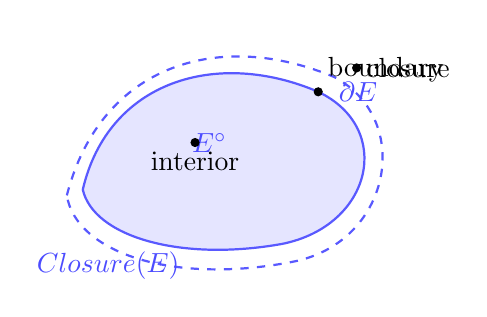
\begin{tikzpicture}[scale=0.92,>=stealth]
  \fill[blue!10]
    (-2.0,-0.5) .. controls (-1.65,1.0) and (-0.15,1.45) .. (1.25,0.85)
    .. controls (2.3,0.35) and (2.0,-1.0) .. (0.75,-1.25)
    .. controls (-0.65,-1.5) and (-1.85,-1.15) .. (-2.0,-0.5);
  \draw[blue!65,thick]
    (-2.0,-0.5) .. controls (-1.65,1.0) and (-0.15,1.45) .. (1.25,0.85)
    .. controls (2.3,0.35) and (2.0,-1.0) .. (0.75,-1.25)
    .. controls (-0.65,-1.5) and (-1.85,-1.15) .. (-2.0,-0.5);
  \draw[blue!65,thick,dashed]
    (-2.22,-0.58) .. controls (-1.75,1.24) and (-0.10,1.72) .. (1.48,1.05)
    .. controls (2.58,0.45) and (2.25,-1.25) .. (0.88,-1.5)
    .. controls (-0.8,-1.82) and (-2.1,-1.35) .. (-2.22,-0.58);

  \node[blue!70] at (-0.25,0.15) {\(E^\circ\)};
  \node[blue!70] at (1.8,0.85) {\(\partial E\)};
  \node[blue!70] at (-1.65,-1.55) {\(\operatorname{Closure}(E)\)};

  \fill[black] (-0.45,0.15) circle (1.8pt);
  \node[below] at (-0.45,0.15) {interior};
  \fill[black] (1.25,0.85) circle (1.8pt);
  \node[above right] at (1.25,0.85) {boundary};
  \fill[black] (1.78,1.18) circle (1.8pt);
  \node[right] at (1.78,1.18) {closure};
\end{tikzpicture}

\caption{Interior, boundary, and closure record different ways points sit
relative to a set: room inside, contact with both sides, and forced inclusion
by arbitrary closeness.}
\label{fig:closure-boundary-interior}
\end{figure}

\begin{dependencies}
\begin{itemize}
  \item \hyperref[def:metric-closure]{Definition: Metric Closure}
\end{itemize}
\end{dependencies}

\begin{definitionbox}{Definition --- Metric Bounded Set}
\begin{definition}[Metric Bounded Set]\label{def:metric-bounded-set}
Let \((X,d)\) be a metric space and let \(A\subseteq X\).  The set \(A\) is
\emph{bounded} if there exist \(x\in X\) and \(R>0\) such that
\[
  d(x,a)\leq R
\]
for every \(a\in A\).
\end{definition}
\end{definitionbox}

\begin{remark*}[Standard quantified statement]
\[
A\text{ is bounded}
\quad\Longleftrightarrow\quad
\exists x\in X\,\exists R>0\,\forall a\in A{:}\ d(x,a)\leq R.
\]
\end{remark*}

\begin{remark*}[Predicate reading]
\[
\operatorname{Bounded}(A,(X,d))
\Longleftrightarrow
\exists x\in X\,\exists R>0\,\forall a\in A{:}\ d(x,a)\leq R
\]
means that \(A\) has finite radius from some center in the metric space.
\end{remark*}

\begin{remark*}[Interpretation]
A bounded set has finite spread from at least one center.  The center is
auxiliary: boundedness records finite reach, not a preferred location.
Important trap: an infinite set can be bounded; for example,
\((0,1)\subseteq\mathbb{R}\) is bounded in the usual metric.
\end{remark*}

\begin{remark*}[Examples]
In \(\mathbb{R}\) with the usual metric, the intervals \((0,1)\),
\([0,1]\), \((a,b)\), and \([a,b]\) are bounded whenever \(a<b\).  The rays
\((0,\infty)\) and \([0,\infty)\), and the whole line \(\mathbb{R}\), are not
bounded.
\end{remark*}

\begin{dependencies}
\begin{itemize}
  \item \hyperref[def:metric-space]{Definition: Metric Space}
\end{itemize}
\end{dependencies}

\begin{figure}[htbp]
\centering
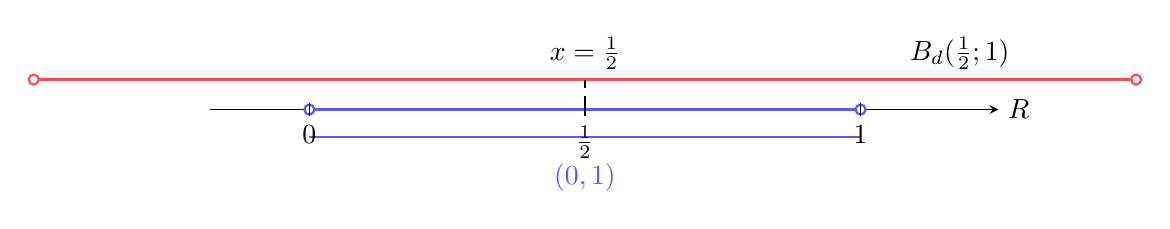
\begin{tikzpicture}[x=7cm,y=1cm,>=stealth]
  \draw[->] (-0.18,0) -- (1.25,0) node[right] {\(\mathbb{R}\)};

  \draw[very thick,blue!65] (0,0) -- (1,0);
  \draw[fill=white,draw=blue!65,thick] (0,0) circle (1.8pt);
  \draw[fill=white,draw=blue!65,thick] (1,0) circle (1.8pt);

  \draw[blue!65,thick] (0,-0.35) -- (1,-0.35)
    node[midway,below=6pt] {\((0,1)\)};

  \draw[red!70,thick] (-0.5,0.38) -- (1.5,0.38);
  \draw[fill=white,draw=red!70,thick] (-0.5,0.38) circle (1.8pt);
  \draw[fill=white,draw=red!70,thick] (1.5,0.38) circle (1.8pt);
  \draw[dashed] (0.5,0.38) -- (0.5,-0.08);
  \node[above] at (0.5,0.38) {\(x=\frac12\)};
  \node[above] at (1.18,0.38) {\(B_d(\frac12;1)\)};

  \foreach \p/\lab in {0/0,0.5/\frac12,1/1}
  {
    \draw (\p,0.08) -- (\p,-0.08);
    \node[below] at (\p,-0.08) {\(\lab\)};
  }
\end{tikzpicture}

\caption{In \(\mathbb{R}\), the interval \((0,1)\) is bounded because every
point of the interval is within distance \(1\) of \(1/2\).}
\label{fig:bounded-interval-r}
\end{figure}

\begin{figure}[htbp]
\centering
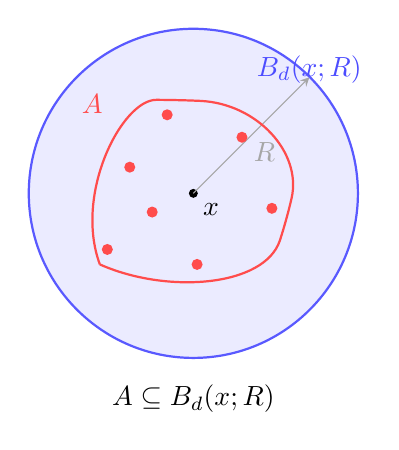
\begin{tikzpicture}[scale=0.95,>=stealth]
  \fill[blue!8] (0,0) circle (2.2);
  \draw[blue!65,thick] (0,0) circle (2.2);
  \node[blue!70] at (1.55,1.65) {\(B_d(x;R)\)};

  \fill[black] (0,0) circle (1.7pt);
  \node[below right] at (0,0) {\(x\)};
  \draw[->,gray!70] (0,0) -- (1.55,1.55);
  \node[gray!70] at (0.95,0.55) {\(R\)};

  \foreach \p in {(-0.85,0.35),(-0.35,1.05),(0.65,0.75),(1.05,-0.2),
                  (0.05,-0.95),(-1.15,-0.75),(-0.55,-0.25)}
  {
    \fill[red!70] \p circle (2.1pt);
  }

  \draw[red!70,thick,rounded corners=8pt]
    (-1.25,-0.95) .. controls (-1.6,0.0) and (-0.95,1.25) .. (-0.2,1.25)
    .. controls (0.85,1.2) and (1.45,0.55) .. (1.25,-0.35)
    .. controls (0.95,-1.25) and (-0.35,-1.35) .. (-1.25,-0.95);
  \node[red!70] at (-1.35,1.2) {\(A\)};

  \node at (0,-2.75) {\(A\subseteq B_d(x;R)\)};
\end{tikzpicture}

\caption{An arbitrary subset \(A\) of a metric space is bounded when all of
its points lie within one finite distance bound from a chosen center.}
\label{fig:bounded-arbitrary-set}
\end{figure}

\begin{theorembox}{Theorem}
\begin{theorem}[Equivalent Boundedness Criterion]
\label{thm:metric-equivalent-boundedness-criterion}
Let \((X,d)\) be a metric space and let \(A\subseteq X\).  Then \(A\) is
bounded if and only if there exist \(x\in X\) and \(R>0\) such that
\[
  d(x,a)<R
\]
for every \(a\in A\).
\hyperref[prf:metric-equivalent-boundedness-criterion]{\textit{Go to proof.}}
\end{theorem}
\end{theorembox}

\begin{remark*}[Standard quantified statement]
\[
A\text{ is bounded}
\quad\Longleftrightarrow\quad
\exists x\in X\,\exists R>0\,\forall a\in A{:}\ d(x,a)<R.
\]
\end{remark*}

\begin{remark*}[Predicate reading]
\[
\operatorname{Bounded}(A,(X,d))
\Longleftrightarrow
\exists x\in X\,\exists R>0\,\forall a\in A{:}\ d(x,a)<R
\]
means that strict and non-strict metric radius bounds define the same
boundedness predicate after enlarging the radius.
\end{remark*}

\begin{remark*}[Interpretation]
Strict and non-strict radius bounds are equivalent after enlarging the radius.
Both express the same finite-spread condition.
\end{remark*}

\begin{dependencies}
\begin{itemize}
  \item \hyperref[def:metric-bounded-set]{Definition: Metric Bounded Set}
\end{itemize}
\end{dependencies}

\begin{theorembox}{Theorem}
\begin{theorem}[Center Independence]\label{thm:metric-bounded-center-independence}
Let \((X,d)\) be a metric space.  If \(A\subseteq X\) and there exist
\(x\in X\) and \(R>0\) such that \(d(x,a)\leq R\) for every \(a\in A\), then
for every \(y\in X\),
\[
  d(y,a)\leq R+d(x,y)
\]
for every \(a\in A\).  Thus boundedness does not depend on the chosen center.
\hyperref[prf:metric-bounded-center-independence]{\textit{Go to proof.}}
\end{theorem}
\end{theorembox}

\begin{remark*}[Standard quantified statement]
\[
\bigl(\forall a\in A{:}\ d(x,a)\leq R\bigr)
\Longrightarrow
\forall y\in X\,\forall a\in A{:}\ d(y,a)\leq R+d(x,y).
\]
\end{remark*}

\begin{remark*}[Predicate reading]
\[
\operatorname{Bounded}(A,(X,d))
\Longrightarrow
\forall y\in X\,\exists S>0\,\forall a\in A{:}\ d(y,a)\leq S
\]
means that boundedness is independent of which ambient point is used as the
center.
\end{remark*}

\begin{remark*}[Interpretation]
Changing centers costs at most the distance between the old center and the
new center.  The triangle inequality transports one finite bound to any other
center.
\end{remark*}

\begin{dependencies}
\begin{itemize}
  \item \hyperref[def:metric-bounded-set]{Definition: Metric Bounded Set}
\end{itemize}
\end{dependencies}

\begin{theorembox}{Theorem}
\begin{theorem}[Subsets of Bounded Sets Are Bounded]
\label{thm:metric-subsets-bounded-sets-bounded}
Let \((X,d)\) be a metric space.  If \(A\subseteq B\subseteq X\) and \(B\) is
bounded, then \(A\) is bounded.
\hyperref[prf:metric-subsets-bounded-sets-bounded]{\textit{Go to proof.}}
\end{theorem}
\end{theorembox}

\begin{remark*}[Standard quantified statement]
\[
A\subseteq B\subseteq X
\;\land\;
B\text{ is bounded}
\Longrightarrow
A\text{ is bounded}.
\]
\end{remark*}

\begin{remark*}[Interpretation]
A subset cannot spread out more than the set containing it.  Any bound for
\(B\) automatically bounds \(A\).
\end{remark*}

\begin{dependencies}
\begin{itemize}
  \item \hyperref[def:metric-bounded-set]{Definition: Metric Bounded Set}
\end{itemize}
\end{dependencies}

\begin{theorembox}{Theorem}
\begin{theorem}[Finite Sets Are Bounded]\label{thm:metric-finite-sets-bounded}
Every finite subset of a metric space is bounded.
\hyperref[prf:metric-finite-sets-bounded]{\textit{Go to proof.}}
\end{theorem}
\end{theorembox}

\begin{remark*}[Standard quantified statement]
\[
A\subseteq X
\;\land\;
A\text{ is finite}
\Longrightarrow
A\text{ is bounded}.
\]
\end{remark*}

\begin{remark*}[Interpretation]
Only finitely many distances must be controlled.  Choosing one center and a
bound larger than all distances from that center captures the whole finite
set.
\end{remark*}

\begin{dependencies}
\begin{itemize}
  \item \hyperref[def:metric-bounded-set]{Definition: Metric Bounded Set}
\end{itemize}
\end{dependencies}

\begin{theorembox}{Theorem}
\begin{theorem}[Finite Unions of Bounded Sets Are Bounded]
\label{thm:metric-finite-unions-bounded-sets-bounded}
Let \((X,d)\) be a metric space, let \(n\in\mathbb{N}\), and let
\(A_1,\ldots,A_n\subseteq X\).  If \(A_1,\ldots,A_n\) are bounded, then
\[
  \bigcup_{k=1}^n A_k
\]
is bounded.
\hyperref[prf:metric-finite-unions-bounded-sets-bounded]{\textit{Go to proof.}}
\end{theorem}
\end{theorembox}

\begin{remark*}[Standard quantified statement]
\[
\bigl(\forall k\in\{1,\ldots,n\}{:}\ A_k\text{ is bounded}\bigr)
\Longrightarrow
\bigcup_{k=1}^n A_k\text{ is bounded}.
\]
\end{remark*}

\begin{remark*}[Interpretation]
Each bounded set has finite spread.  A finite union still has only finitely
many centers and bounds to absorb into one sufficiently large bound.
\end{remark*}

\begin{dependencies}
\begin{itemize}
  \item \hyperref[def:metric-bounded-set]{Definition: Metric Bounded Set}
  \item \hyperref[thm:metric-bounded-center-independence]{Theorem: Center Independence}
\end{itemize}
\end{dependencies}

\begin{theorembox}{Theorem}
\begin{theorem}[Boundedness via Diameter]\label{thm:metric-boundedness-via-diameter}
Let \((X,d)\) be a metric space and let \(A\subseteq X\) be nonempty.  Then
\(A\) is bounded if and only if there exists \(C>0\) such that
\[
  d(a,b)\leq C
\]
for all \(a,b\in A\).
\hyperref[prf:metric-boundedness-via-diameter]{\textit{Go to proof.}}
\end{theorem}
\end{theorembox}

\begin{remark*}[Standard quantified statement]
\[
A\neq\varnothing
\Longrightarrow
\Bigl(
A\text{ is bounded}
\Longleftrightarrow
\exists C>0\,\forall a,b\in A{:}\ d(a,b)\leq C
\Bigr).
\]
\end{remark*}

\begin{remark*}[Predicate reading]
\[
\operatorname{Bounded}(A,(X,d))
\Longleftrightarrow
\exists C>0\,\forall a,b\in A{:}\ d(a,b)\leq C
\]
means that a nonempty metric set is bounded exactly when all pairwise
distances in the set are uniformly bounded.
\end{remark*}

\begin{remark*}[Interpretation]
For nonempty sets, boundedness can be measured internally: all pairwise
distances must be uniformly bounded.  This is the diameter viewpoint.
\end{remark*}

\begin{dependencies}
\begin{itemize}
  \item \hyperref[def:metric-bounded-set]{Definition: Metric Bounded Set}
  \item \hyperref[def:metric-diameter]{Definition: Diameter}
\end{itemize}
\end{dependencies}

\begin{theorembox}{Theorem}
\begin{theorem}[Closure of a Bounded Set Is Bounded]
\label{thm:metric-closure-bounded-set-bounded}
Let \((X,d)\) be a metric space.  If \(A\subseteq X\) is bounded, then
\(\operatorname{Closure}(A)\) is bounded.
\hyperref[prf:metric-closure-bounded-set-bounded]{\textit{Go to proof.}}
\end{theorem}
\end{theorembox}

\begin{remark*}[Standard quantified statement]
\[
A\text{ is bounded}
\Longrightarrow
\operatorname{Closure}(A)\text{ is bounded}.
\]
\end{remark*}

\begin{remark*}[Interpretation]
Passing to the closure may add limit points, but it does not create points
arbitrarily far away.  A slightly enlarged bound still captures the closure.
\end{remark*}

\begin{dependencies}
\begin{itemize}
  \item \hyperref[def:metric-bounded-set]{Definition: Metric Bounded Set}
  \item \hyperref[def:metric-closure]{Definition: Metric Closure}
\end{itemize}
\end{dependencies}

\begin{theorembox}{Theorem}
\begin{theorem}[Compact Sets Are Bounded]\label{thm:metric-compact-sets-bounded}
Every compact subset of a metric space is bounded.
\hyperref[prf:metric-compact-sets-bounded]{\textit{Go to proof.}}
\end{theorem}
\end{theorembox}

\begin{remark*}[Standard quantified statement]
\[
K\subseteq X
\;\land\;
K\text{ is compact}
\Longrightarrow
K\text{ is bounded}.
\]
\end{remark*}

\begin{remark*}[Interpretation]
The open balls centered at any fixed point cover the compact set as their
radii grow.  Compactness reduces this cover to finitely many radii, and the
largest one bounds the set.
\end{remark*}

\begin{dependencies}
\begin{itemize}
  \item \hyperref[def:metric-bounded-set]{Definition: Metric Bounded Set}
\end{itemize}
\end{dependencies}

\begin{theorembox}{Theorem}
\begin{theorem}[Totally Bounded Sets Are Bounded]
\label{thm:metric-totally-bounded-sets-bounded}
Every totally bounded subset of a metric space is bounded.
\hyperref[prf:metric-totally-bounded-sets-bounded]{\textit{Go to proof.}}
\end{theorem}
\end{theorembox}

\begin{remark*}[Standard quantified statement]
\[
A\subseteq X
\;\land\;
A\text{ is totally bounded}
\Longrightarrow
A\text{ is bounded}.
\]
\end{remark*}

\begin{remark*}[Interpretation]
A totally bounded set can be covered by finitely many balls of one fixed
radius.  A finite collection of bounded balls has finite overall spread, so
the set is bounded.
\end{remark*}

\begin{dependencies}
\begin{itemize}
  \item \hyperref[def:metric-bounded-set]{Definition: Metric Bounded Set}
  \item \hyperref[thm:metric-finite-unions-bounded-sets-bounded]{Theorem: Finite Unions of Bounded Sets Are Bounded}
\end{itemize}
\end{dependencies}
